%% packages
\documentclass{article}
\usepackage[a4paper, left=2.0cm, right=2.0cm, top=3.5cm]{geometry}
\usepackage[ngerman]{babel}
\usepackage{graphicx}
\usepackage{multicol}
\usepackage{amssymb}
\usepackage{titlesec}
\usepackage{wrapfig}
\usepackage{blindtext}
\usepackage{lipsum}
\usepackage{caption}
\usepackage{listings}
\usepackage{fancyhdr}
\usepackage{nopageno}
\usepackage{authblk}
\usepackage{amsmath} % tons of math stuff
\usepackage{mathtools} % e.g. alignment within matrix
%\usepackage{bm} % provides shorthand for bold in math mode
\usepackage{dsfont} % \mathds makes double stroke digits
\usepackage{esdiff} % provides \diff
%\usepackage[ISO]{diffcoeff}
\usepackage{xcolor}
\usepackage{csquotes} % e.g. provides \enquote
\usepackage[separate-uncertainty=true]{siunitx} % units
\usepackage{xcolor} % colored text
\usepackage[l3]{csvsimple}
\usepackage{subcaption}
\usepackage{physics}
\usepackage{hyperref}
\usepackage{nameref}
\hypersetup{colorlinks=true, linkcolor=black, pdfhighlight={/N}}
\usepackage{tcolorbox}
\usepackage{amsthm}
\usepackage{gensymb} % add \degree in math mode?
\usepackage{newunicodechar} % define custom unicode characters
\usepackage{booktabs}
\usepackage{subcaption}

% \sisetup{
%   scientific-notation = auto,  % Automatically use scientific notation for large/small numbers
%   output-exponent-marker = \text{e}  % (optional) for formatting the exponent symbol
% }



%\fancyhf[]{}

%% custom stuff
% own units
\DeclareSIUnit \VSS {\ensuremath{V_\mathrm{SS}}}
\DeclareSIUnit \VS {\ensuremath{V_\mathrm{S}}}
\DeclareSIUnit \Veff {\ensuremath{V_\mathrm{eff}}}
\DeclareSIUnit \Vpp {\ensuremath{V_\mathrm{pp}}}
\DeclareSIUnit \Vp {\ensuremath{V_\mathrm{p}}}
\DeclareSIUnit \VRMS {\ensuremath{V_\mathrm{RMS}}}
\DeclareSIUnit \ASS {\ensuremath{A_\mathrm{SS}}}
\DeclareSIUnit \AS {\ensuremath{A_\mathrm{S}}}
\DeclareSIUnit \Aeff {\ensuremath{A_\mathrm{eff}}}
\DeclareSIUnit \App {\ensuremath{A_\mathrm{pp}}}
\DeclareSIUnit \Ap {\ensuremath{A_\mathrm{p}}}
\DeclareSIUnit \ARMS {\ensuremath{A_\mathrm{RMS}}}

% change subsection numbering to capital letters
\newcommand{\subsectionAlph}{ \renewcommand{\thesubsection}{\arabic{section}.\Alph{subsection}} }
% change subsection numbering to lowercase letters
\newcommand{\subsectionalph}{ \renewcommand{\thesubsection}{\arabic{section}.\alph{subsection}} }
% change subsubsection numbering to lowercase letters
\newcommand{\subsubsectionalph}{ \renewcommand{\thesubsubsection}{\arabic{section}.\arabic{subsection}.\alph{subsubsection}} }
% own fig. that works with multicols
\newenvironment{Figure}
  {\par\medskip\noindent\minipage{\linewidth}}
  {\endminipage\par\medskip}
\newcommand*{\inputPath}{./plot} % prepend this command to the argument of all input commands
\graphicspath{ {./figure/}{../plot/}{../assets} }
% own enviroment for definitions
\newenvironment{definition}[1]
{\begin{quote} \noindent \textbf{\textit{#1\ifx&#1& \else : \fi}} \itshape}
{\end{quote}}

\newunicodechar{°}{\degree}


% own commands
% \newcommand{\rarr}{$\to\,$} %A$\,\to\,$B
\newcommand{\defc}{black}
\newcommand{\colorT}[2][blue]{\color{#1}{#2}\color{\defc}}
\newcommand{\redq}{\color{red}(?)\color{\defc}}
\newcommand{\question}[1]{\colorT[purple]{\textbf{(#1)}}}
\newcommand{\todo}[1]{\colorT[red]{\textbf{(#1)}}}
\newcommand{\mr}{\mathrm}

%% preparation
\begin{titlepage}
    \title{Praktikum Atome, Moleküle, kondensierte Materie \\ Versuch 442: Laser}
    \author[1]{Michael Vogt\thanks{s65mvogt@uni-bonn.de}}
    \affil[1]{Uni Bonn}
    %\date{\today}
\end{titlepage}


%% document
\begin{document}

\pagenumbering{gobble}
\maketitle
\tableofcontents
\newpage
\pagenumbering{arabic}

\pagestyle{fancy}
\fancyhead[R]{\thepage}
\fancyhead[L]{\leftmark}

\section*{TODO}
\begin{itemize}
  \item \todo{\enquote{Aufgaben} durchgehen und ins Protokoll aufnehmen}
  
\end{itemize}

\section*{Einleitung}
Durch diesen Versuch soll die grundlegende Funktionsweise von Lasern anhand eines Helium-Neon-Lasers verstanden werden.
Zunächst werden Wellenlänge und Polarisation des Lichts gemessen und anschließend die Aufspaltung in verschiedene
Moden genauer untersucht. Zum stabilen Betrieb des Lasers wird eine optische Diode aufgebaut.

\section{Aufbau des Lasers}
Zunächst wird der Laser aufgebaut und justiert. Seine fundamentalen Bestandteile sind
\begin{enumerate}
  \item das \textbf{Lasermedium}, ein mit HeNe gefülltes Volumen. Durch Anlegen einer hohen Spannung kann das Helium
  auf den $2^1S_0$-Zustand angeregt und seine Energie durch inelastische Stöße an Neon-Atome abgeben,
  welche dadurch auf den 3s-Zustand, der ein ähnliches Energieniveau hat, angeregt werden (siehe Abb. \ref{fig:hene-level}).
  Dieser Zustand ist metastabil bezüglich spontaner Emission, wodurch es zu einer \textit{Besetzungsinversion} kommt: 
  Es befinden sich mehr Atome im höheren 3s-Zustand als im Grundzustand.
  \todo{Laserübergang beschreiben}
  % durch stimulierte Emission
  % kann jedoch der 3s$\rightarrow$2p-Übergang sehr häufig stattfinden.
  Dieser Prozess wird als \textbf{optisches Pumpen} bezeichnet.
  \item Ein \textbf{Resonator} aus zwei Spiegeln, der einen großen Teil des entstehenden Lichts vielfach durch das
  Lasermedium leitet. Dadurch können Photonen des 3s$\rightarrow$2p-Übergangs, der sonst nur selten durch
  spontane Emission stattfinden würde, denselben Übergang wieder
  stimulieren und weitere Photonen freisetzen. Es findet also ein verstärkender Prozess statt, der dem Laser
  seinen Namen gibt: \textit{Light Amplification Through Stimulated Emission of Radiation}.
\end{enumerate}

\begin{figure}[h]
  \centering
  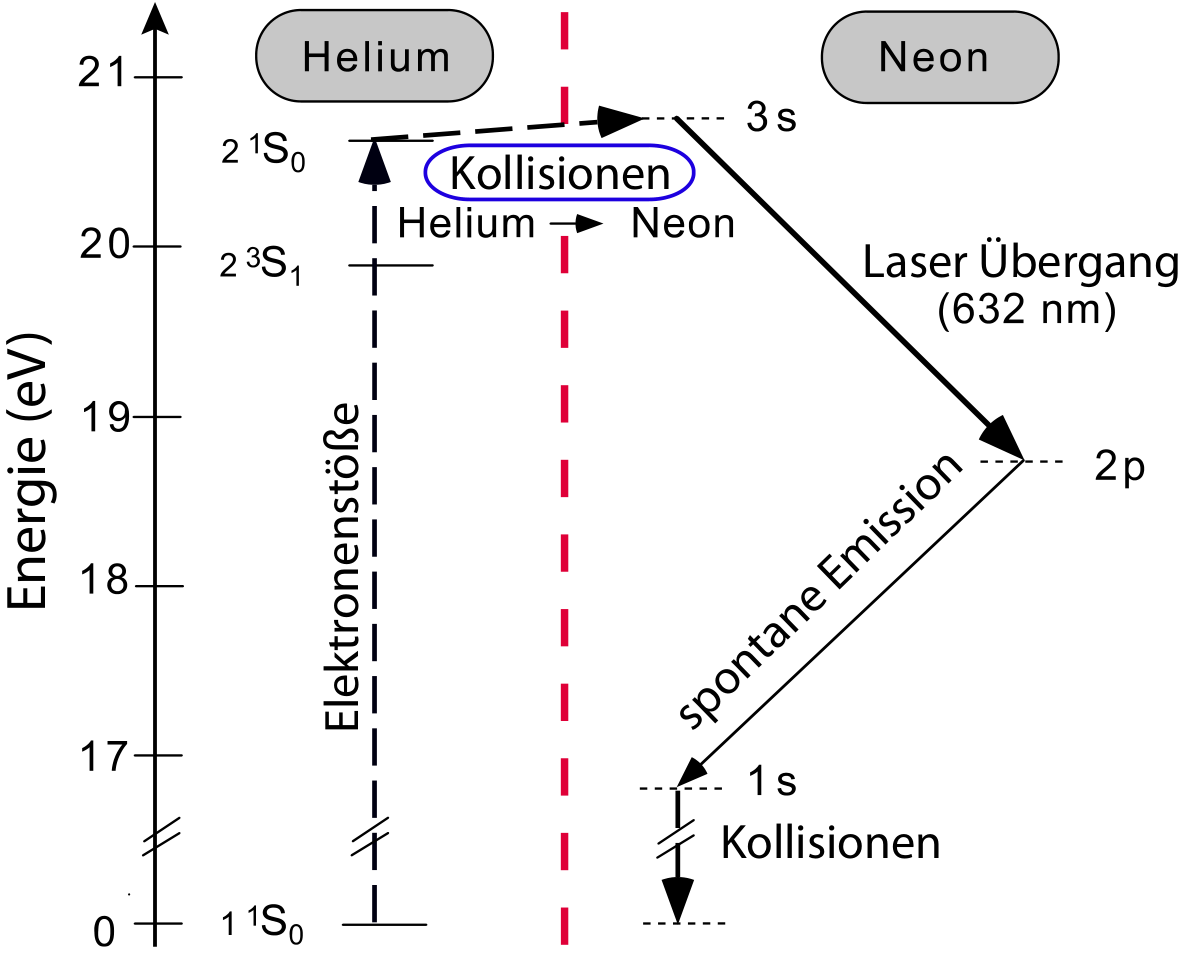
\includegraphics[width=0.5\textwidth]{hene-level}
  \caption{Für den Laserbetrieb relevant Energienievaus von Helium und Neon. \cite{Anleitung}}
  \label{fig:hene-level}
\end{figure}

\section{Wellenlänge und Polarisation}
Zunächst werden Wellenlänge und Polarisation des Laserlichts gemessen.
Es wurde ab hier ein anderer Aufbau als der zuvor beschriebene verwendet, da ich am zweiten Tag den Versuch als Teil
einer Dreiergruppe fortführte.
Die Aufbauten funktionieren grundlegend gleich und unterscheiden sich nur in den Details der Strahlführung.

\subsection{Wellenlänge}
Anhand der Ablenkung des Laserlichts an einem Transmissionsgitter, welches in den Strahlverlauf gestellt wird,
kann dessen Wellenlänge bestimmt werden.
Es gilt die Gittergleichung
\begin{equation}
  n\lambda = d(\cos \alpha - \cos \beta_n)
\end{equation}
wobei $\alpha$ der Winkel des Lasers und $\beta_n$ der Winkel der $n$-ten Beugungsordnung zur Gitternormalen ist. 
Daraus folgt die Geradengleichung
\begin{equation}
  n = n(\cos\beta) = \frac{d}{\lambda} (\cos \alpha - \cos \beta)
\end{equation}
also gilt für die Steigung $m$
\[
  m = -\frac{d}{\lambda} \iff \lambda = -\frac{d}{m}
\]

Hier galt $d=\todo{Wert}. $Die gemessenen Ordnungen sind in Tab. \ref{tab:gitter-fit} gezeigt.
Eine Geradenanpassung von $n$ in Abhängigkeit von $\cos \beta$ liefert die Gleichung
\[
  n(\cos\beta) = \todo{Werte}
\]
also $m = \todo{Wert}$ und $\lambda = \todo{Wert}$. \todo{Vergleich mit erwarteter Wellenlänge} 

\subsection{Polarisierung}
Als nächstes soll die Polarisierung des Laserlichts gemessen werden. Im Lasermedium wird zunächst unpolarisiertes Licht
erzeugt. Dieses verlässt das Medium jedoch durch Brewsterfenster, welche nur eine bestimmte Polarisationsrichtung durchlassen
\todo{stimmt das? Brewsterfenster erklären.}.

Zur Messung der Polarisation wird das Licht durch einen Polarisator auf eine Photodiode geschickt
und die zur Lichtintensität proportionale Spannung mithilfe eines Oszilloskops gemessen.
Bei vollständig linear polarisiertem Licht und einem idealen Polarisator
ist der Zusammenhang zwischen Intensität $I$ und Winkel $\alpha$ des
Polarisators zur Vertikalen durch das \textit{Malus'sche Gesetz} gegeben:
\begin{equation}
  I(\alpha) = I_0 \cos^2(\alpha - \alpha_0)
\end{equation}
mit $I_0$ der Lichtintensität vor dem Polarisator und $\alpha_0$ der Polarisationsrichtung des Lichts (zur Vertikalen).

Im Allgemeinen kann der $\cos^2$-Verlauf im Vergleich zum Malus'schen Gesetz gestaucht sein, wenn das Licht nicht vollständig
polarisiert ist:
% erreicht der Verlauf nicht mehr die maximale oder die verschwindende Intensität, sondern ist auf einen kleineren Bereich
% eingeschränkt:
\begin{equation}
  I(\alpha) = U_\mr{min} + (U_\mr{max}-U_\mr{min}) \cos^2(\alpha - \alpha_0) \label{eq:malus-real}
\end{equation}
\todo{begründen wo das herkommt}
Hier wurde Spannung $U$ anstatt Intensität $I$ verwendet, da die Spannung hier die
zur Intensität proportionale gemessene Größe ist.

Bei Sättigung der Diode würde der $\cos^2$-Verlauf oberhalb der Maximalspannung der Diode \enquote{abgeschnitten} werden
und damit nicht mehr \eqref{eq:malus-real} entsprechen. Es wurde daher sichergestellt, dass keine Sättigung auftritt.
\todo{abschlusswiderstand erklälren?}
Der Polarisator auf verschiedene Winkel in regelmäßigen Abständen eingestellt und jeweils die Spannung notiert.
Diese Werte sind in Tab. \ref{tab:polarisation} gezeigt und in Abb. \ref{fig:polarisation} aufgetragen, zusammen
mit einer $\chi^2$-Anpassung nach \eqref{malus-real}. Diese liefert die Parameter
\todo{Werte}, 
\todo{Polarisationsrichtung vergleichen},

% Der Polarisationsgrad PG ist definiert durch 
% \begin{equation}
%   \mr{PG} \coloneq \frac{I_\parallel - I_\perp}{I_\parallel + I_\perp}
%   = \frac{U_\parallel - U_\perp}{U_\parallel + U_\perp}
%   = \frac{U_\mr{max} - U_\mr{min}}{U_\mr{max} + U_\mr{min}} 
% \end{equation}
% wobei 
Für den Polarisationsgrad PG gilt 
\begin{equation}
  \mr{PG} = \frac{U_\mr{max} - U_\mr{min}}{U_\mr{max} + U_\mr{min}} = \todo{Wert einfüllen}
\end{equation}
\todo{Diskutieren wenn nicht vollständig polarisiert}



\clearpage
\section{Fazit}



\clearpage
\section{Anhang}



\clearpage
\begin{thebibliography}{9}

\bibitem{Anleitung}
\textit{Physikalisches Praktikum Teil IV -- Versuchsbeschreibungen}, Universität Bonn, 10.10.2024



\end{thebibliography}

\end{document}

